\chapter{Tables, Figures and Other Features}
This chapter shows example of picture and also serves to populate the different lists: list of figures, list of tables, bibliography, and glossary.

\section{Tables}
This section contains examples of tables.

\begin{table}[H]
\centering
\begin{tabular}{ccc}
\toprule
name & weight & food \\ 
\midrule
mouse	& 10 g	& cheese \\
cat	& 1 kg	& mice \\
dog	& 10 kg	& cats \\
t-rex	& 10 Mg	& dogs \\
\bottomrule 
\end{tabular}
\caption[A floating table]{A floating table.}
\label{tab:esempio}
\end{table}

\section{Figures}
This section contains examples of figures.

\begin{figure}[H] 
\centering 
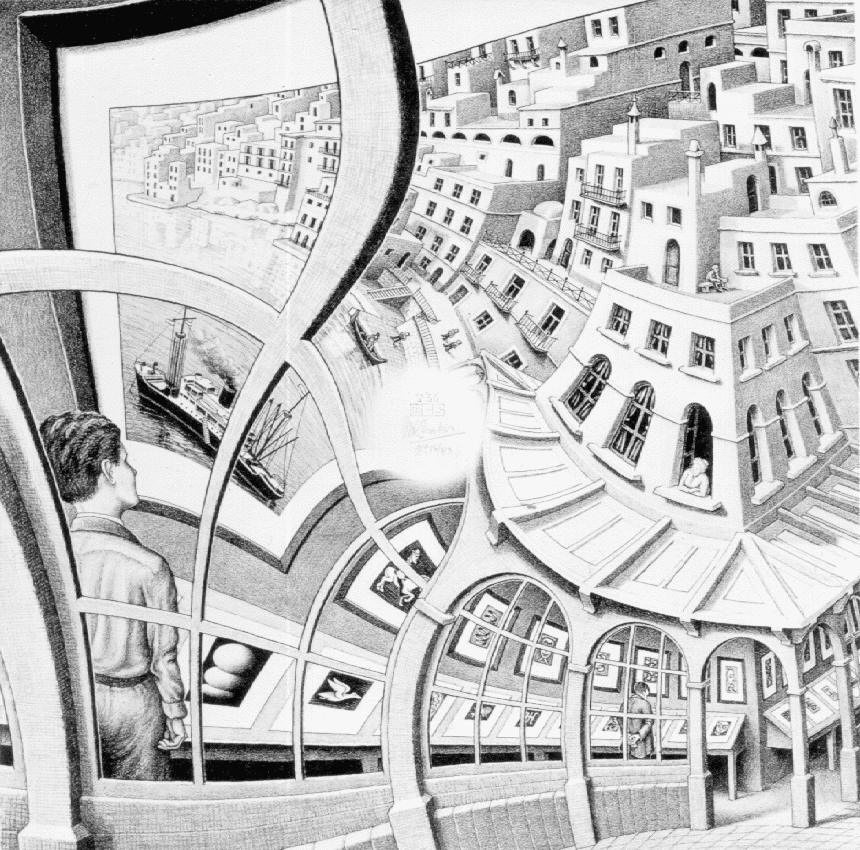
\includegraphics[width=0.5\columnwidth]{galleria_stampe} 
\caption[A floating figure]{A floating figure (the lithograph \emph{Galleria di stampe}, of M.~Escher, got from \url{http://www.mcescher.com/}).}
\label{fig:galleria} 
\end{figure}

\begin{figure}[H]
	\centering
	\begin{subfigure}[b]{0.45\textwidth}
		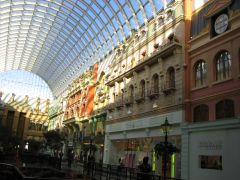
\includegraphics[width=\textwidth]{lorem}
		\caption{A gull}
		\label{fig:lorem}
	\end{subfigure}
	~ %add desired spacing between images, e. g. ~, \quad, \qquad, \hfill etc. 
	%(or a blank line to force the subfigure onto a new line)
	\begin{subfigure}[b]{0.45\textwidth}
		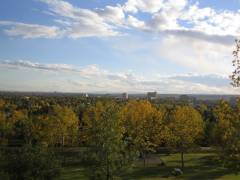
\includegraphics[width=\textwidth]{ipsum}
		\caption{A tiger}
		\label{fig:ipsum}
	\end{subfigure}
	~ %add desired spacing between images, e. g. ~, \quad, \qquad, \hfill etc. 
	%(or a blank line to force the subfigure onto a new line)
	\begin{subfigure}[b]{0.45\textwidth}
		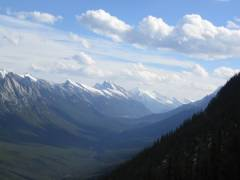
\includegraphics[width=\textwidth]{dolor}
		\caption{A mouse}
		\label{fig:dolor}
	\end{subfigure}
	~ %add desired spacing between images, e. g. ~, \quad, \qquad, \hfill etc. 
	%(or a blank line to force the subfigure onto a new line)
	\begin{subfigure}[b]{0.45\textwidth}
		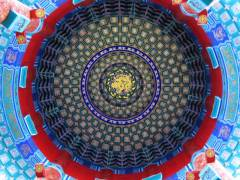
\includegraphics[width=\textwidth]{sit}
		\caption{A mouse}
		\label{fig:sit}
	\end{subfigure}
	\caption{Example subcaption}\label{fig:animals}
\end{figure}



